\documentclass[12pt]{article}

\pagestyle{empty}
\setlength{\topmargin}{0in}
\setlength{\headheight}{0in}
\setlength{\topsep}{0in}
\setlength{\textheight}{9in}
\setlength{\oddsidemargin}{0in}
\setlength{\evensidemargin}{0in}
\setlength{\textwidth}{6.5in}

\usepackage{palatino, graphicx,amssymb}

\newcommand{\ds}{\displaystyle}
\newcommand{\vs}[1]{\vspace{#1in}}
\renewcommand{\vss}[1]{\vspace*{#1in}}
\newcommand{\bvec}{{\mathbf b}}
\newcommand{\cvec}{{\mathbf c}}
\newcommand{\dvec}{{\mathbf d}}
\newcommand{\evec}{{\mathbf e}}
\newcommand{\fvec}{{\mathbf f}}
\newcommand{\qvec}{{\mathbf q}}
\newcommand{\uvec}{{\mathbf u}}
\newcommand{\vvec}{{\mathbf v}}
\newcommand{\wvec}{{\mathbf w}}
\newcommand{\xvec}{{\mathbf x}}
\newcommand{\yvec}{{\mathbf y}}
\newcommand{\zvec}{{\mathbf y}}
\newcommand{\zerovec}{{\mathbf 0}}
\newcommand{\real}{{\mathbb R}}
\newcommand{\twovec}[2]{\left[\begin{array}{r}#1 \\ #2
    \end{array}\right]}
\newcommand{\ctwovec}[2]{\left[\begin{array}{c}#1 \\ #2
   \end{array}\right]}
\newcommand{\threevec}[3]{\left[\begin{array}{r}#1 \\ #2 \\ #3
  \end{array}\right]}
\newcommand{\cthreevec}[3]{\left[\begin{array}{c}#1 \\ #2 \\ #3
    \end{array}\right]}
\newcommand{\fourvec}[4]{\left[\begin{array}{r}#1 \\ #2 \\ #3 \\ #4
    \end{array}\right]}
\newcommand{\cfourvec}[4]{\left[\begin{array}{c}#1 \\ #2 \\ #3 \\ #4
    \end{array}\right]}
\newcommand{\fivevec}[5]{\left[\begin{array}{c}#1 \\ #2 \\ #3 \\ #4 \\
                                 #5 \\
    \end{array}\right]}
\newcommand{\mattwo}[4]{\left[\begin{array}{rr}#1 & #2 \\ #3 & #4 \\ \end{array}\right]}
\renewcommand{\span}[1]{\text{Span}\{#1\}}
\newcommand{\bcal}{{\cal B}}
\newcommand{\ccal}{{\cal C}}
\newcommand{\scal}{{\cal S}}
\newcommand{\wcal}{{\cal W}}
\newcommand{\ecal}{{\cal E}}
\newcommand{\coords}[2]{\left\{#1\right\}_{#2}}
\newcommand{\gray}[1]{\color{gray}{#1}}
\newcommand{\lgray}[1]{\color{lightgray}{#1}}
\newcommand{\rank}{\text{rank}}
\newcommand{\col}{\text{Col}}
\newcommand{\nul}{\text{Nul}}

\begin{document}

\noindent
{\bf Mathematics 227} \\ 
{\bf Lab 4, Due: November 28, 2018}

\bigskip
\noindent
{\bf Instructions:} The exercises here should be completed in groups
of 2 or 3 students with one write-up submitted from each group.

\medskip
When I recently googled the phrase ``linear algebra,'' Google told me
there were about 36.5 million results and that the Wikipedia page was
the one most likely to be useful to me.  How does Google decide to
recommend that page above all the others?  Simply said, Google
computes a quantity called PageRank for each page on the Internet.
Pages with a higher PageRank are deemed to be more valuable.  The key
to computing PageRank lies in an algorithm, which we'll study in this
lab.  

\medskip One could determine the importance of a web page by allowing
people to vote for their favorite web pages.  However, Google wants
their rankings to be free of any human bias so it examines the
structure of the Internet itself to rank pages.  Here's the idea:  if
my home page is valuable, many other pages will link to it.  Of course, I
could game the rankings by creating lots of pages that link to my home
page.  So Google views a page as being more valuable when valuable
pages link to it.  For instance, if three of my friends link to my
home page, that means three people think I have a valuable page.  But
if {\tt nytimes.com}, {\tt amazon.com}, and {\tt beyonce.com} link to
me, that probably means more people will find my page to be valuable
so I should have a higher PageRank.

\medskip
Here's how to compute PageRank.  Each webpage has a certain amount of
PageRank that we denote by $x_i$.  Each page divides its PageRank into
equal portions, one for each outgoing link.  Each page then gives one
portion of its PageRank to each page it links to.  A page's PageRank
is then the sum of all the PageRank it receives from pages that link
to it.  Let's look at an example.

\bigskip
\begin{enumerate}
\item Suppose that our Internet only has three pages with links as
  shown below.  Page 2 only links to page 1 so it gives all of its
  PageRank $x_2$ to Page 1.  Page 3 has two outgoing links so it
  divides its PageRank $x_3$ into two equal pieces and gives half its
  PageRank $x_3/2$
  to Page 1.  The PageRank $x_1$ is therefore
  $$
  x_1 = x_2 + \frac 12 x_3.
  $$
  \begin{center}
    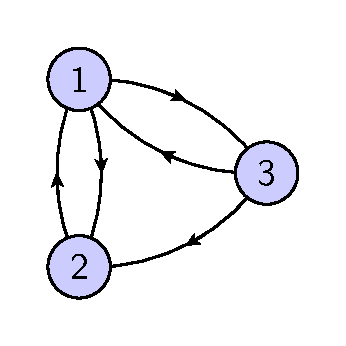
\includegraphics{google-intro.eps}
  \end{center}
  Find similar expressions for $x_2$ and $x_3$.

  \vs{1}
  If we write $\xvec = \threevec{x_1}{x_2}{x_3}$, find the ``Google
  matrix'' $G$ such that $\xvec = G\xvec$.

  \vs{1}
  Explain why $G$ is a stochastic matrix.  Why will this always be the
  case for any Internet, assuming that each page has outgoing links?

  \vs{1}
  By looking at this web, which web page do you think is most
  valuable?  Explain your response.

  \vs{1}
  Is $G$ a positive matrix?  Explain why or why not.

  \vs{1}
  The PageRank vector is defined by the equation $\xvec =
  G\xvec$ and any scalar multiple of $\xvec$ will satisfy this
  equation too.  Of course, we are only interested in the relative
  values of the PageRank (that is, which pages have the highest
  PageRank) so this doesn't need to concern us.

  \newpage
  However, we are now exactly in the situation where we can apply the
  Perron-Frobenius theorem, which says that there is a unique
  steady-state vector $\qvec$ with all positive entries.  Find this
  steady-state vector $\qvec$, which will be the PageRank vector.

  \vs{1}
  Which is the page with the highest PageRank?  Which is the page with
  the smallest PageRank?  Does this agree with your intution?  If not,
  take a moment to figure out why not.

  \vs{1}
  The problem is that Google currently knows about 100 trillion
  ($10^{14}$ pages) so the real Google matrix is 100 trillion $\times$
  100 trillion.  Finding the PageRank vector by finding a basis for
  the eigenspace $E_1$ by row reduction is not computationally
  feasible.  However, the Perron-Frobenius theorem tells us that any
  Markov chain will converge to the PageRank vector $\qvec$!

  \medskip
  If you visit the page {\tt http://gvsu.edu/s/0To}, you will find
  some Sage code that will be helpful for this lab.  In particular,
  you should evaluate the first cell to load in some functions.  In
  particular, there is a function {\tt markov\_chain(A, x0, N)} that
  prints $N$ vectors in the Markov chain defined by a stochastic
  matrix $A$ and initial state vector $\xvec_0$.

  \medskip
  Verify that a Markov chain beginning with $\xvec_0 = \threevec100$
  converges to the PageRank vector $\qvec$.  What do you find after 10
  terms?  

  \vs{1}
\item Consider the Internet shown below.  Find the Google matrix $G$
  and its PageRank vector using a Markov chain.

  \begin{center}
    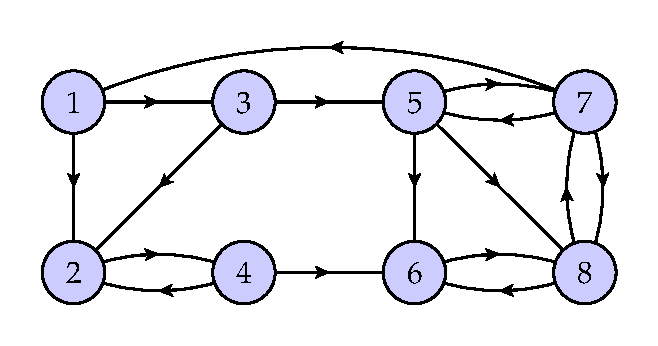
\includegraphics{google-irreducible.eps}
  \end{center}

  What do you find for the PageRank vector?  Which page is most
  valuable?  Which page is least valuable?

  \vs{1}
\item Now consider the Internet shown below and write the Google
  matrix.

  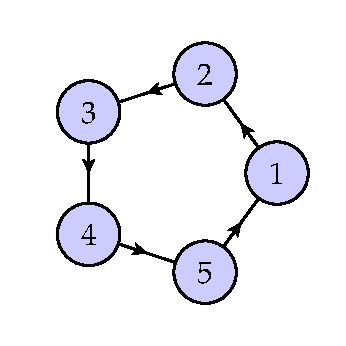
\includegraphics{google-cyclic.eps}

  Is $G$ a positive matrix in this case?  Explain why or why not.

  \vs{0.75}
  What happens to a Markov chain that begins with the initial state
  $\xvec_0 = \fivevec10000$?

  \vs{1}
  Look closely at this Internet and state what you feel the PageRank
  vector should be in this case?

  \vs{1}
\item Consider the following Internet and write its Google matrix.

  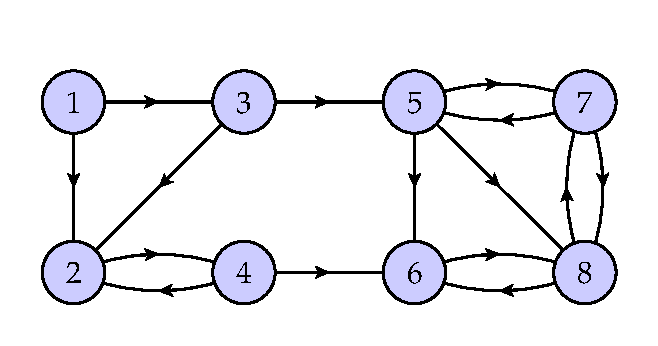
\includegraphics{google-reducible.eps}

  Is the Google matrix positive?  Explain why or why not.

  \vs{1}
  What happens if you build a Markov chain using this matrix?  Why is
  this not satisfactory?

  \vs{1}
\item As the last two examples show, the Google matrix is not always
  positive so the Perron-Frobenius theorem does not always apply.
  This means that a Markov chain may not converge or it may converge
  to a vector with zero entries.  Because of this reason, Google
  modifies the Google matrix so that the modified matrix is positive.
  Here's what happens.

  If there are $n$ web pages, define the matrix
  $$
  H_n =
  \left[
    \begin{array}{cccc}
      \frac1n & \frac1n & \cdots & \frac1n \\
      \frac1n & \frac1n & \cdots & \frac1n \\
      \vdots & \vdots & \ddots & \vdots \\
      \frac1n & \frac1n & \cdots & \frac1n \\
    \end{array}
  \right].
  $$
  This would correspond to an Internet in which every page is linked
  to every other page, including itself.  We now define a modified
  Google matrix $G'$ by choosing a parameter $\alpha$, which is a trade
  secret but is suspected to be close to $\alpha=0.85$, and defining
  $$
  G'= \alpha G + (1-\alpha)H_n,
  $$
  or, if $\alpha = 0.85$,
  $$
  G'=0.85 G + 0.15 H_n.
  $$
  In other words, $G'$ is obtained by mixing 85\% of $G$ with 15\% of
  $H_n$.  You may use the Sage command {\tt
    modified\_Google\_matrix(G, alpha)} to produce $G'$.

  Go back and revisit the Internet having five pages linked together
  in a cycle.  Construct the modified Google matrix $G'$ with $\alpha
  = 0.85$.  Explain why this is a positive matrix.

  \vs{1}
  What do you now find for the PageRank vector using $G'$?  Does this
  agree with what you think the PageRank vector should be?

  \vs{1}
  Revisit the second Internet we considered that had eight pages and
  construct the modified Google matrix.  What do you find for the
  PageRank vector now?  Which page is most important and which is
  least important?

  \vs{1}

\item Markov chains can always be thought of statistically so the
  PageRank vector has a statistical interpretation.  Suppose we begin
  on one page.  Every second, we randomly follow a link on the current
  page to another page with equal probability.  Suppose we do this
  until the end of time.  The PageRank vector gives us the fraction of
  time that we spend on each page.  Clearly, we will spend more time
  on more important pages.

  When we modify the Google matrix, we make the modification that,
  85\% of the time, we follow a randomly chosen link on our current
  page, and 15\% of the time, we leap to some other randomly chosen page
  on the Internet.  The PageRank vector again tells us what fraction
  of time we spend on each page.

  

  

  
  
    
  

  

\end{enumerate}






\end{document}